\chapter{Experiment 1: Invalid execution traces}\label{sec:ch4}

\info{intro}

\section{Method}

The lightweight version from the previous chapter is only able to test one specific
bug. The bug itself is created manually by modifying the \gls{sut}. Now,
this lightweight version needs to be automated to automatically generate a test
for every transition from a specification.

With every transition, it is possible to reach a state or stay in the current
state. To check \textit{Rebel} specifications, the state to reach with a transition needs
to be defined. As mentioned before, the goal of model checking is to find a
state which is reachable with some properties which do not hold
~\cite[p.~5]{stoel_storm_vinju_bosman_2016}. Thus defining only the reachable
state is not enough, the properties of interest for a transition needs to be
specified. Each property is different per transition, so these properties should
be different for the defined state. For example for the \textit{close}
transition, we want to check whether it is possible to have a closed account
where the balance is not equal to zero, for the transition \textit{withdraw} we
want to check whether a negative balance can be achieved with the transition.

To conclude, with this approach we are testing the opposite of the preconditions.
Thus what is not possible according to the specification is tested.

\subsection{Evaluation criteria}\label{sec:ch4-eval-criteria}

\subsubsection{Bugs}
Since we are testing with this approach the opposite of the preconditions, thus
what should be not possible according to the specification. It is expected to
find bugs in the \gls{sut} where it is possible to perform the opposite of a
transition. So faults can be found like preconditions which are not properly
generated. An example of this is the manually created bug
(\autoref{fig:ch3-res-codegenakka-account}) for the lightweight version.

\subsubsection{Efficiency}
In this approach is checking used to check what is not possible according to the
specification. Therefore, the same tested transition should be tested in the
\gls{sut}. To test all transitions from the account specification, it may take
longer since some transactions require an initial state for which transitions
need to be performed to reach this state.

\subsubsection{Coverage}
The experiment is going to generate a test for all transitions. Therefore,
it is expected to test all the transitions of a specification. With the criteria
bugs, we discussed the expectation to find faults in not properly generated
preconditions. This may lead to the inability to test transitions. For example,
when a failure (incorrect preconditions) occurs during reaching the initial
state of the \textit{withdraw} transition. This leads to the inability to test
the \textit{withdraw} transition.

\section{Approach}
The testing approach is a well-known approach in mutation testing. Mutation testing is
a fault-based testing technique, which generates faulty programs by syntactic
changes to the original program.~\cite[p.~1]{jia2011analysis} The set of faulty
programs are called mutants, each mutant contains a different syntactic change.
In our case, only one mutant is generated. A test suite for a program is used to
determine whether the faulty programs are detected. A mutant is killed when it
is detected by the test suite. The mutant is in our case killed when the result
from the \gls{smt} solver and the \gls{sut} are the same. we are using the same
approach from \autoref{sec:ch3} to compare the results of the \gls{smt} solver and
\gls{sut}.

Mutation testing generates a mutant based on
mutation operator, which is a transformation rule that generates a mutant from
the original program.~\cite[p.~3-4]{jia2011analysis} The mutation operator for
our approach is Negate Conditionals Mutator~\cite{pitmutators}, this operator
belongs to the type relational operator
replacement~\cite[p.~688]{king1991fortran}.

The testing approach is illustrated in \autoref{fig:mutated-checking}. The first
step is to start with a \textit{Rebel} specification, which is in our case the already
existing account specification. When the specifications are defined, the
specifications are being built, \textit{i.e.}, \gls{csts} are
produced of these specifications. Using these \gls{csts}, the code generator generates
the code, which is then the \gls{sut}.

The test case generator can be used to test the \gls{sut} when the \gls{sut} is generated
from the \gls{csts}. The \gls{csts} of the specifications are traversed by the test case
generator to generate a test for each transition. The test case generator
generates tebl files for transitions to use checking.

To test the \gls{sut}, the test case generator performs a similar transition
as used within checking in the \gls{sut}. Finally, the results from checking and the
performed transition in the \gls{sut} are compared.

\begin{figure}[h!]
  \centering
  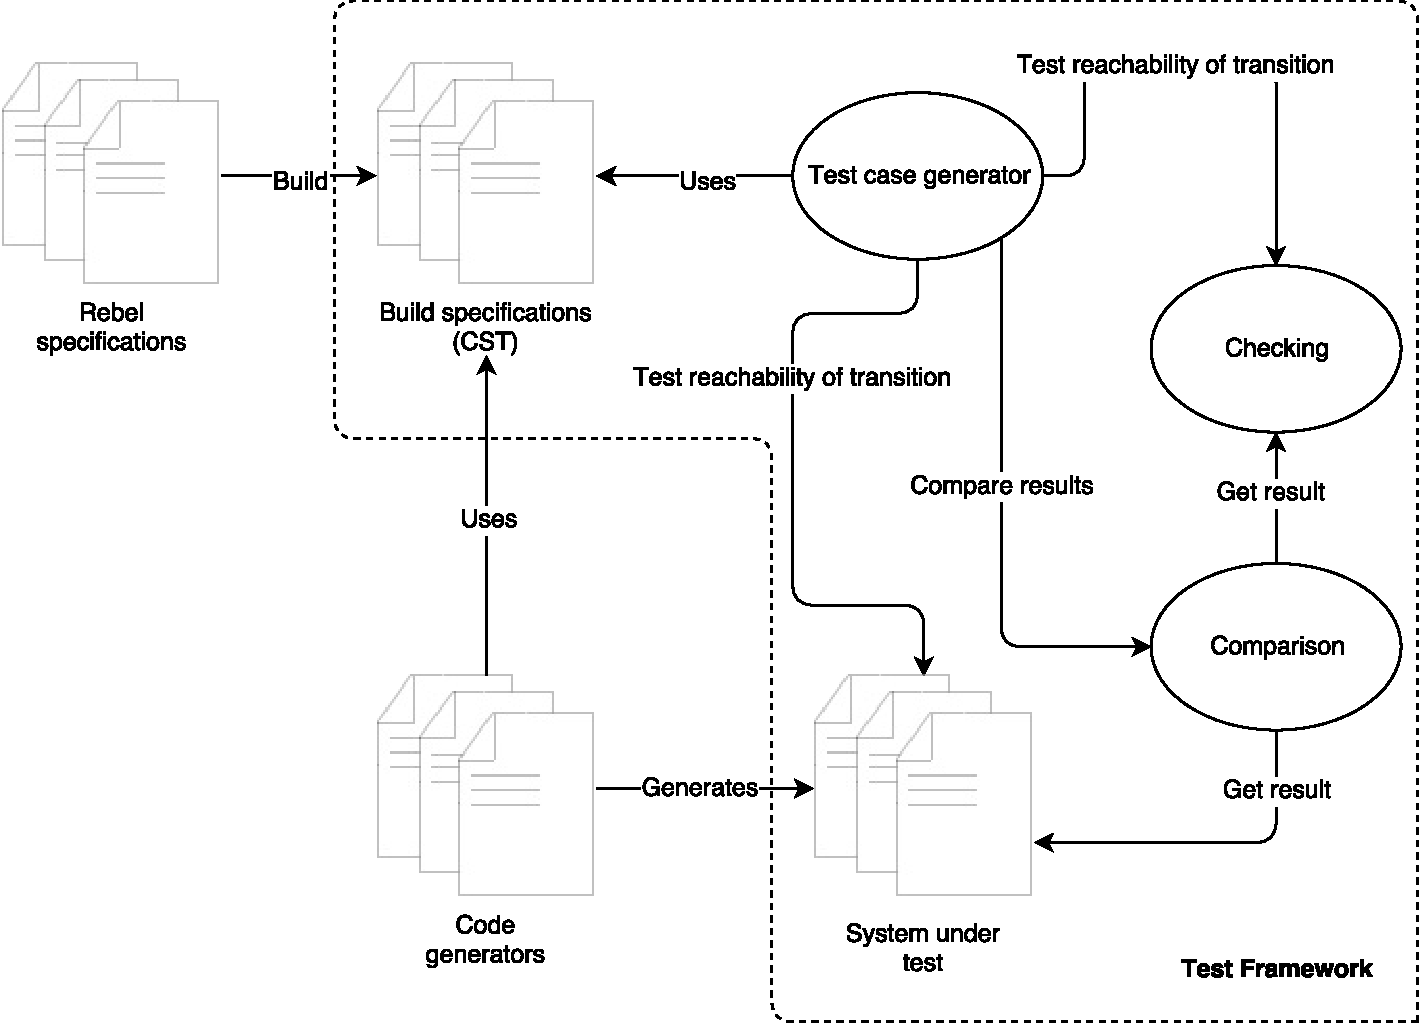
\includegraphics[width=\linewidth{}]{figures/mutated-checking-diagram.pdf}
  \caption{Testing approach with checking}\label{fig:mutated-checking}
\end{figure}
\FloatBarrier

\subsection{Checking}
Only expressions which contain a reference to the specification fields needs to
be replaced since it is only possible in tebl to specify the reachable state
with the properties of interest (these properties are not part of the
transition).

Earlier the definition of the \textit{close} event transition was given in
\autoref{fig:account-close-event} which contains the following statement
\code{this.balance == EUR 0.00;}. When this statement is translated to tebl
with a negated conditional, it looks as follows
\code{balance != EUR 0.00;}. Thus the replaced conditional is the opposite
condition of the statement defined in the \textit{close} transition.

Replacing conditionals to negated conditionals is done for all conditionals with
relational operators. The chosen mutation operator Negate Conditionals Mutator
will replace conditionals according to the replacement table in
\autoref{fig:table-replacement-conditions}.

\begin{table}[h!]
\centering
\begin{tabular}{cc}
\toprule
\textbf{Actual expression} & \textbf{Translated expression} \\ \midrule
!=                         & ==                             \\
==                         & !=                             \\
\textgreater               & \textless=                     \\
\textgreater=              & \textless                      \\
\textless                  & \textgreater=                  \\
\textless=                 & \textgreater                   \\ \bottomrule
\end{tabular}
\caption{Conditionals replacement~\cite{pitmutators}}\label{fig:table-replacement-conditions}
\end{table}
\FloatBarrier

\subsection{\gls{sut}}
The conditionals for the transition in the \gls{sut} are also replaced.
Although, it is not necessary to replace always the conditionals. For some
transitions is an initial state required, \textit{e.g.}, to execute the transition unblock
of the account specification, the account should be in the state blocked. So an
initial state needs to be constructed for some transitions. Of course, the \gls{smt}
solver can construct its initial state to reach a state.

The definition of the \textit{deposit} transition is given in
\autoref{fig:account-deposit-event} and contains the following statement in the
preconditions \code{amount > EUR 0.00;}. First, the initial state needs to be
constructed which is the state opened. Following is the replacement of the conditionals, the
replaced precondition from the \textit{deposit} transition looks as follows
\code{amount > EUR 0.00;}. The \textit{deposit} transition needs then to be
performed in the \gls{sut}.

To perform the \textit{deposit} transition, the transition parameters for this
transition must be determined satisfying replaced conditionals. The transition
parameter for the \textit{deposit} transition, amount, should be less
than or equal to 0 euro. Therefore, are generators implemented to generate
values satisfying the negated conditionals. For example, the following
transition parameter is generated to be used in the \textit{deposit} transition
\code{"amount": "EUR -2.00"}.

\begin{sourcecode}[h!]
\begin{lstlisting}[]
event deposit(amount: Money) {
	preconditions {
		amount > EUR 0.00;
	}
	postconditions {
		new this.balance == this.balance + amount;
	}
}
\end{lstlisting}
\caption{\textit{deposit} event definition from specification}\label{fig:account-deposit-event}
\end{sourcecode}
\FloatBarrier

\section{Results}

\subsection{Codegen-Akka}

For this experiment, we are testing the generator Codegen-Akka. The results
of this test run are shown in \autoref{fig:ch5-res-codegenakka-account}. As shown
in this table, the tests for four transitions are successful and the tests for
the other three transitions are failed.

\begin{table}[h!]
\centering
\begin{tabular}{cc}
\toprule
\textbf{Transition to test} & \textbf{Transition} \\ \midrule
openAccount                 & \cmark{}            \\
withdraw                    & \xmark{}            \\
deposit                     & \xmark{}            \\
interest                    & \cmark{}            \\
block                       & \cmark{}            \\
unblock                     & \cmark{}            \\
close                       & \xmark{}            \\ \bottomrule
\end{tabular}
\caption{Results: testing account specification transitions}\label{fig:ch5-res-codegenakka-account}
\end{table}
\FloatBarrier

\section{Analyse}

\subsection{Codegen-Akka}

% https://github.com/cwi-swat/ing-rebel-generators/commit/999e6b40307a79fb245ace15375c27461c92374e
\subsubsection{Bug: closing an account with balance}\label{sec:bug-close-account}
When this automated version of checking is executed, it produces some false
positives. After investigating the tests for the transitions, the test for the \textit{close}
transition seems not be successful (see \autoref{fig:result-close-account}).
The model checker states that the state is not reachable (the same tebl file is
generated as in \autoref{fig:tebl-closed-account}). It seems to be that the
state is reachable in the \gls{sut}.

\begin{sourcecode}[h!]
\begin{lstlisting}[]
Test transition close
opened -> close -> closed
generated close test in |project://rebel-core/examples/simple_transaction/
  OpenedToClosedViaCloseTest.tebl|

Reachability transition: false
Execute transition result: true
Result successful transition test: false
\end{lstlisting}
\caption{Result run}\label{fig:result-close-account}
\end{sourcecode}
\FloatBarrier

When we take a look at the account in the \gls{sut}, it looks as
follows in \autoref{fig:closed-account-json}. The state of the account is in
closed, which is correct according to the specification, but the balance of the
account is 52 euro. In \autoref{fig:account-close-event} we already discussed
the event  definition of the \textit{close} transition, which is that the
balance should be equal to zero. From this, we can conclude that we have
discovered a bug in the \gls{sut}.

\begin{sourcecode}[h!]
\begin{lstlisting}[]
[{
	"_id": 17592186045441,
	"_version": 2,
	"_status": "CLOSED",
	"accountNumber": {
		"iban": "NO3627716652225"
	},
	"balance": {
		"value": 52.00,
		"currency": "EUR"
	}
}]
\end{lstlisting}
\caption{account state in json}\label{fig:closed-account-json}
\end{sourcecode}
\FloatBarrier

Now we know that we have discovered a bug, we want to know why this behaviour
occurs and whether it is due to the generated code from the specification. The
method which handles the \textit{close} transition has the following check in
\autoref{fig:java-notequal-check}. The if statement checks whether the balance
of the account is not equal to 0 euro. The condition in the if statement is not
satisfied with the balance of 52 euro. That is why the exception
\textit{BuildCASTransactionException} is not thrown.

\begin{sourcecode}[h!]
\begin{lstlisting}[language=Java]
if(! (isNotEqual(_entity.getBalance(), Money.of(org.joda.money.CurrencyUnit.of("EUR"), 0.00)))) {
  throw new BuildCASTransactionException("Predicate did not hold: CloseTransaction: this.balance ==
  EUR 0.00");
}
\end{lstlisting}
\caption{Code in Java}\label{fig:java-notequal-check}
\end{sourcecode}
\FloatBarrier

The question right now is, how is the above code generated. After taking a look at the synthesization of
expression, the expressions from \textit{Rebel} are not properly synthesized. The
synthesization for an equal expression for the type \textit{Money} or \textit{Percentage} looks as
follows in \autoref{fig:rascal-datomic-synthesize-equal}. The expression is
synthesized to the method \textit{isNotEqual} with two parameters.

\begin{sourcecode}[h!]
\begin{lstlisting}[]
private str g(e:(Expr)`<Expr lhs> == <Expr rhs>`, tmap t) = "isNotEqual(<g(lhs, t)>, <g(rhs, t)>)"
  when isType(t, lhs, (Type)`Percentage`) || isType(t, lhs, (Type)`Money`);
\end{lstlisting}
\caption{Generate equal expression in Rascal}\label{fig:rascal-datomic-synthesize-equal}
\end{sourcecode}
\FloatBarrier

So the expression is not properly synthesized, and it should be synthesized to
\textit{isEqual} instead of \textit{isNotEqual}. With this modification, it
is not possible anymore to close an account with some balance. This also applies
to other statements which use the equal operator.

% https://github.com/cwi-swat/ing-rebel-generators/pull/6
\subsubsection{Bug: deposit with a maximum amount}\label{sec:bug-compile-max-deposit}

The automated checking is implemented with the ability to first start the
\gls{sut} and then run the tests against it. For a new test run, the
specification has changed a little bit. It is now possible to only deposit with
a maximum amount (see \autoref{fig:java-deposit-maxamount}). After the code is
generated, the testing framework is not able to start the system. There is a
compile error as you can see in
\autoref{fig:java-result-lessthan-compile-error}, the binary operator "$<$"
is not applicable on the type \textit{org.joda.money.Money}. The compile error
is thrown by the source code from \autoref{fig:java-lessthan-compile-error},
which is part of the method which handles the \textit{deposit} transition.

% less than, not compilable. Duplicate method for greaterThan should be lessThan

\begin{sourcecode}[h!]
\begin{lstlisting}[]
event deposit(amount: Money) {
	preconditions {
		amount < EUR 250.00;
	}
	postconditions {
		new this.balance == this.balance + amount;
	}
}
\end{lstlisting}
\caption{\textit{deposit} event definition from specification}\label{fig:java-deposit-maxamount}
\end{sourcecode}
\FloatBarrier

\begin{sourcecode}[h!]
\begin{lstlisting}[]
Error:(63, 23) java: bad operand types for binary operator '<'
  first type:  org.joda.money.Money
  second type: org.joda.money.Money
\end{lstlisting}
\caption{\textit{deposit} event definition from specification}\label{fig:java-result-lessthan-compile-error}
\end{sourcecode}
\FloatBarrier

\begin{sourcecode}[h!]
\begin{lstlisting}[language=Java]
if(! ((amount < Money.of(org.joda.money.CurrencyUnit.of("EUR"), 200.00)))) {
  throw new BuildCASTransactionException("Predicate did not hold: DepositTransaction:
  amount < EUR 250.00");
}
\end{lstlisting}
\caption{Code in Java}\label{fig:java-lessthan-compile-error}
\end{sourcecode}
\FloatBarrier

The functions for the synthesization, which generates a part of
\autoref{fig:java-lessthan-compile-error}, are shown in
\autoref{fig:rascal-datomic-synthesize-lessthan}. Also here are the \textit{Rebel}
expression not properly synthesized. The default expression with the binary
operator "$<$" is properly synthesized to an expression with three expressions,
the left-hand and right-hand side expression and the binary operator "$<$".
As discussed before, the binary operator "$<$" doesn't work with
\textit{org.joda.money.Money}. Thus the default method to synthesize expressions
with the binary operator "$<$" cannot be used for the type
\textit{org.joda.money.Money}.

On line number 1 of \autoref{fig:rascal-datomic-synthesize-lessthan} is the
synthesization method of the expression with the binary operator "$>$" shown.
This method is already defined before in the corresponding file. To conclude,
this method should synthesize expressions with the binary operator "$<$".

\begin{sourcecode}[h!]
\begin{lstlisting}[]
private str g(e:(Expr)`<Expr lhs> \> <Expr rhs>`, tmap t) = "isGreaterThan(<g(lhs, t)>, <g(rhs, t)>)"
  when isType(t, lhs, (Type)`Percentage`) || isType(t, lhs, (Type)`Money`);
private str g(e:(Expr)`<Expr lhs> \< <Expr rhs>`, tmap t) = "(<g(lhs, t)> \< <g(rhs, t)>)";
\end{lstlisting}
\caption{Generate equal expression in Rascal}\label{fig:rascal-datomic-synthesize-lessthan}
\end{sourcecode}
\FloatBarrier

\section{Evaluation}\label{sec:ch4-evaluation}

\subsection{Bugs}
In \autoref{sec:ch4-eval-criteria} we discussed the expectations of the criteria
bugs. We expected to find bugs in the \gls{sut} where it is possible to perform
the opposite of a transition. Thus it is expected to find bugs where the
preconditions are not properly generated.

With this experiment, we have found a bug in the \gls{sut}, which was
discussed in \autoref{sec:bug-close-account}. The other bug is out of scope
since the \gls{sut} is not able to compile. With the bug from
\autoref{sec:bug-close-account}, it is possible that the final state closed is
reached where the preconditions of the \textit{close} transition do not hold.
So as expected, we did find a bug in performing the opposite of a transition
where the preconditions were not properly generated.

\info{traces are possible}

\subsection{Efficiency}
For the criteria efficiency, it is expected to check what is not possible
according to the specification, i.e. testing the same transition in checking as
well as in the \gls{sut}.

A part of the generated test for a transition is checking, which is used to test
the state to reach with the replaced preconditions. So, in this experiment, we
are testing what should be not possible according to the
specification. The expectation is that the same transitions with checking should
be performed on the \gls{sut}. However, the result of the checking from the
\gls{smt} solver varies, \textit{e.g.}, an opened account can be reached by the
\textit{openAccount} transition or by the transition \textit{openAccount} and
\textit{withdraw}. Thus the test framework is not able to perform the same
transitions on the \gls{sut} as the transitions from checking.

With testing all transitions from the account specification, it is possible that
testing may take longer. As expected, this is the case since due to the initial
state transitions are more executed and tested. To conclude, the testing process
may take longer to test all the transitions.

\subsection{Coverage}
It is expected for this criteria to test all the transitions of the
specification since the experiment generated tests for all transitions.

In the experiment, after the checking, a transition
is performed in the \gls{sut}. In this experiment, it is unknown whether the
performed transition with its parameters in the \gls{sut} is the same as the
transition computed by the \gls{smt} solver. This causes some false positives in the
test run. Also, it is difficult to play like the \gls{smt} solver; it is unknown which
result the \gls{smt} solver will give. The \gls{smt} solver is also smarter/better in checking
the satisfiability of a given constraints.

Failure occurring along the way in constructing the initial state of a transition
may lead to the inability to test transitions. Unfortunately, there does not
seem to be any faults in here.

\section{Conclusion}
In this experiment is the account specification used to test the \gls{sut}.
This experiment generates automatically tests for transitions.

A part of
the generated test for a transition is checking, which is used to test the state to
reach with the replaced preconditions. So, in this experiment, we are
testing what should be not possible according to the specification. The result
of the checking from the \gls{smt} solver varies, \textit{e.g.}, an opened account can be
reached by the \textit{openAccount} transition or by the transition
\textit{openAccount} and \textit{withdraw}.

After the checking, a transition
is performed in the \gls{sut}. In this experiment, it is unknown whether the
performed transition with its parameters in the \gls{sut} is the same as the
transition computed by the \gls{smt} solver. This causes some false positives in the
test run. Also, it is difficult to play like the \gls{smt} solver; it is unknown which
result the \gls{smt} solver will give. The \gls{smt} solver is also smarter/better in checking
the satisfiability of a given constraints.

To conclude, the checking used in this experiment tests only the states, regardless of which transitions are
being performed, and testing the \gls{sut} focuses more on testing transitions.

With this experiment, we have found a bug in the \gls{sut}, which was
discussed in \autoref{sec:bug-close-account}. The other bug is out of scope
since the \gls{sut} is not able to compile. The found bug belongs to the category
injected code since the generated code for the precondition is wrong. In this
case, the final state closed is reached where the preconditions of the \textit{close}
transition do not hold. So the theory for this found bug is
$\forall e s_{1} \to s_{2}, s_{2} \gets s_{1}, pre(e)$.

% claims from finding the bugs.

% \begin{itemize}
% \item je bent in een state gekomen via een preconditie
% \item de transitie zelf verander de pre conditie niet, (de preconditie geldt dan in de postconditie)
% \item het was de laatste

% \item $\forall e s1 \to s2, in s2 geldt pre(e) \lor (! pre(e) \land post(e))$
% \item $\forall e s1 \to s2, in s2 post(e)$
% % of?
% \item $\forall e s1 \to s2, s2 alleen bereikbaar via (1), dan pre(e)$
% \end{itemize}

\section{Threats to validity}

\subsection*{Limited specifications}
In the conducted experiment is the account specification account used
to test the \gls{sut}. With this experiment and specification,
we did find a bug in the code generators.

The used account specification in this experiment is quite simple. With the use
of more interacting specifications, the chance is bigger to find faults in the code
generators since the specifications are interacting with each other.

\subsection*{Invalid execution trace}
The conducted experiment test only what should be not possible according to the
specification. It is also important to test whether the \gls{sut} is conform to the
specification, \textit{i.e.}, testing the valid execution trace.
